\section{Performance Metrics for WebRTC}


%% 
%% Leave first page empty
\thispagestyle{empty}

This section describes metrics to monitor the performance of WebRTC topologies, WebRTC environments require a specific approach and metrics to define how the protocol behaves in different scenarios. 

Some issues affect how WebRTC performs, these range from the resources available in the peers to the state of the link. In the following chapters we describe some of them that we use in our study cases.

Other different issues come with the ability of WebRTC to share link capacity with other ongoing sessions or different traffic when having parallel calls. This might be a problem for the quality of the session and one reason for call failure.

There are two different type of metrics, from one side metrics related to network performance and on the other side those to the host. Some of them are going to be similar to rate and congestion but others might be more close to the performance of the actual API implementation on the browser.

\subsection{Simple Feedback Loop}

Traditionally, real time media communication always rely on inelastic traffic, this type of traffic has low tolerance to error as packets should always arrive in time for playback, this is more important than having 100\% packet delivery rate. Elastic traffic is common in applications that do not require real time data to be sent and is tolerant to delay, having better data delivery performance compared to inelastic traffic.

%With real time media applications, congestion directly affects in traffic delivery rate and performance, if the media generation rate is lower than the available channel capacity there is no need for rate adaption. However, losses and available capacity of the link can vary on time requiring adaptation from the sender side. This adaptation is done by analyzing the receiver feedback packets sent to the sender, this technique is called simple feedback loop.

 \begin{figure}[h]
  \centering
    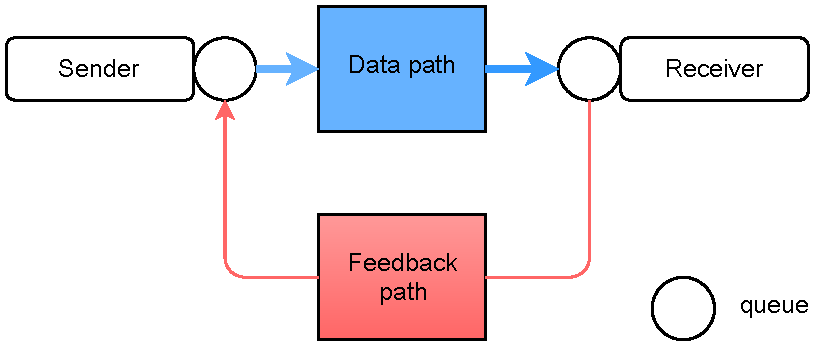
\includegraphics[width=0.8\textwidth]{./figures/simplefeedback.pdf}
      \caption[Multimedia feedback loop]{Multimedia feedback loop.}
	\label{fig:feedbackloop}
\end{figure}

Figure~\ref{fig:feedbackloop} shows a simplified feedback model for multimedia communication, the feedback path carries messages with the link characteristics that help the sender to adjust its congestion mechanisms. Those feedback messages are sent periodically by the receiver and are very important to repost the status of the link.

%\subsection{Congestion control in real time media communication}
%
%Congestion control decisions in real time media communication are done periodically with the data retrieved from various sources, such as the feedback loop. This data helps the protocol to trigger special mechanisms that can modify the traffic shape of the peers that participate in the call. The factors that interact in this decision-making process are the metrics exposed in the following chapters.
%
%Different schemes can be given in congestion control mechanisms.
%
%Sender-driven rate adaptation is one of the methods to control the congestion of the link, his mechanism requires the sender to be aware of the status of the path. Different algorithms will then evaluate the congestion on the path and take decisions on how to send the media.
%
%Receiver-driven rate adaptation requires the receiver to study the status of the network and provide the best rate values back to the source of the data. Those values are then applied to the source of the traffic.
%
%Network-driven rate adaptation is the ability of the network to provide congestion information to the peers of a call about the capacity available and future variables. Once both peers have the new information of network rate, provided by some element of the network, they will be able to adjust to the new condition.
%
%There are two different types of congestion control: congestion avoidance and congestion mitigation.   
%
%Congestion avoidance is done before the link undergoes heavy congestion. Small congestion conditions can be detected by closely evaluating delay, jittering and different metrics. When doing congestion avoidance small changes occur in the sender to better adapt the rate.
%
%However, congestion mitigation is the action performed once the link is already handling heavy congestion. In this case, actions taken by the algorithms are drastic in order to mitigate congestion.
% 
% \begin{figure}[h]
%  \centering
%    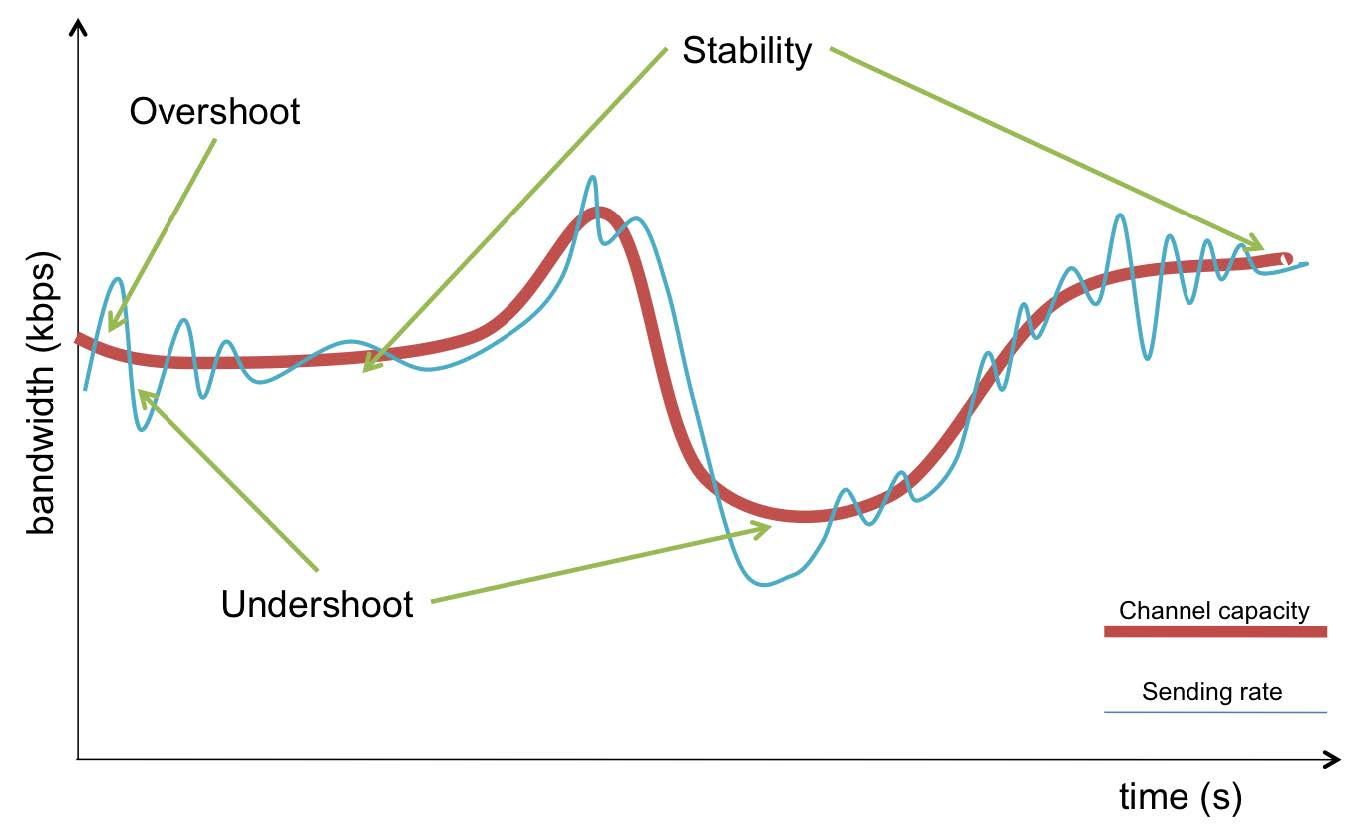
\includegraphics{./figures/rateadaptation.jpg}
%      \caption[Rate adaptation modes. Source~\cite{varunthesis}]{Rate adaptation modes. Source~\cite{varunthesis}.}
%	\label{fig:rateadaptation}
%\end{figure}
%
%When congestion is detected in the path, rate control algorithms operate in three different modes (Figure~\ref{fig:rateadaptation}): {\it overshoot}, {\it undershoot} and {\it stability}.
%
%Overshoot appears when the sending rate exceeds the capacity of the link, this mode of rate adaptation usually produces more congestion on the path and extra packet losses.
%
%Undershoot is the opposite behavior to Overshoot, it is given when heavy congestion appear on the link and packet losses occur. This produces a sudden conservative rate to avoid more losses and mitigate congestion.
%
%Stability is given when the capacity of the link is the same for a certain period of time, bandwidth rate may fluctuate but it will finally converge to the stable channel capacity on the path.
%
\subsection{Network metrics}

Metrics defined in this chapter are only related to those provided by the network, those metrics usually trigger the congestion mechanisms in WebRTC changing the behavior of the stream according to the constraints on the link~\cite{rtpusageIETF}~\cite{alvestrandCongestion2012}. 

With real time media applications, congestion directly affects in traffic delivery rate and performance, if the media generation rate is lower than the available channel capacity there is no need for rate adaption. However, losses and available capacity of the link can vary on time requiring adaptation from the sender side to the new constraints. This adaptation is done by analyzing the receiver feedback packets sent to the sender using the simple feedback loop.

Three global factors are considered when analyzing network links: {\it loss}, {\it bandwidth} and {\it delay}.

\subsubsection{Losses}

Loss rate indicate packet losses during the transmission over the path. Usually packet losses affect directly the quality of a call. In WebRTC, packet loss is a direct indicator of the media quality of the ongoing WebRTC transmission. 

%There are two types of losses, bit-error losses and congestion. Bit-error losses appear randomly and affect some packets, those packets are automatically discarded as the data has been corrupted, this type of error occurs randomly and cannot be predicted easily. Over use of a link produces losses due to congestion of a path, those errors can be anticipated by using congestion mechanisms. 

%Some delayed packets should also be considered as losses, in real-time applications, as they are not useful anymore for the ongoing connection, those packets are not collected in the stats as losses and are directly discarded in the receiver. In WebRTC, loss rate directly affect to the ongoing transmission as the delay range that we can tolerate is very low before the quality of the call deteriorates, some data-driven WebRTC connections can tolerate some more delay. In overall, Loss Rate is used as a key metric to choose a better path route when having high loss. This indicator is manly attached to link quality.
When monitoring WebRTC calls we use packet loss as an indicator to adapt the media constraints, we can use the output provided by the packet loss to reduce the frames per second that {\it GetUserMedia} has configured to obtain the media. 

Losses can also trigger some specific JavaScript mechanism that monitors the call quality and analyzes the overall ongoing session, this mechanism could average some other metrics in order to give an output value of the media quality. Given this value, the constraints regarding video size, frames per second and bandwidth limit can be configured into the {\it GetUserMedia} and {\it PeerConnection}�APIs for better adaptation to the path conditions.

WebRTC uses RTCP packets for control and monitoring on the ongoing stream~\cite{rtcpIETF}. In RTCP losses are reported in the feedback message, this metric does not include discarded packets by the protocol.

Losses are calculated in a period of time, with this we shall be able to see how much loss rate we have in a certain path.

\begin{equation}
	\frac{PKT_{loss}(T) - PKT_{loss}(T-1)}{PKT_{received}(T) - PKT_{received}(T-1) + PKT_{loss}(T) - PKT_{loss}(T-1)}
	\label{eq:PKTloss}
\end{equation}

Equation~\ref{eq:PKTloss} calculates the estimated packet loss we have on the link. This operation is done periodically by our statistical API.

\subsubsection{Round-Trip Time (RTT) and One-Way Delay (OWD)}

Delay in a link can be measured form different perspectives, One-Way Delay (OWD) \nomenclature{OWD}{One-Way Delay} indicates the time it takes for a packet to move from one peer to the other peer, this time includes different delays that are produced along the link. OWD is calculated form the time taken to process the packet in both sides (building and encoding), the lower layer delay in the client (interface and intra-layering delay), queuing delay (from the multiple buffers in the path) and propagation delay (speed of light). The sum of all those delays compose the total one-way delay.

\begin{equation}
	OWD = delay_{propagation} + delay_{queues} + delay_{serialization} + delay_{processing}	
	\label{eq:owd}
\end{equation}

Considering the structure of WebRTC, one of the most important delays that we have to measure and study is the processing delay, as our applications are executed in a multiple layer structure. Running on top of the browser can affect the performance compared to other technologies that run directly over the OS. Delays in our case are symmetric as we are continuously sending and receiving media, low delay is important in order to reproduce the streams in the best quality possible and avoid uncomfortable communication. 

OWD and RTT \nomenclature{RTT}{Round-Trip Time} measurements are included in the standard RTCP specification, in order to calculate those metrics, timestamp from sender and receiver is needed in the reports~\cite{rtcpIETF}. Sender Report (ST) timestamp is saved in the sender, meanwhile, the receiver returns the same timestamp in the Receiver Report (RR) that goes back to the origin. With those, we are able to calculate the RTT using the following Equation~\ref{eq:rtt}.

\begin{equation}
\label{eq:rtt}
\begin{split}
&RTT = TS_{RR} - TS_{SR} -T_{Delay}\\
 \quad &TS_{RR} \text{: Local timestamp at reception of last Receiver Report} \\
 \quad &TS_{SR}�\text{: Last Sender Report timestamp} \\
 \quad &T_{Delay} \text{: Receiver time period between SR reception and RR sending in the sender}
\end{split}
\end{equation}

We can calculate the RTT using the data given by the {\it Stats API} in WebRTC, this metric is important to be monitored as it indicates the time delay on the link and the response of the media when received.

Calculating OWD requires both machines clock to be accurately synchronized and can be complicated, we try to accomplish this but usually OWD delay can be defined as $\frac{RTT}{2}$. 

\subsubsection{Throughput}

Throughput is a key metric for testing the performance of WebRTC environments, this value is going to describe how much capacity of the link is taken by each {\it PeerConnection}. It is complex though, as there are still no fully functional QoS mechanisms implemented in WebRTC at this time. The throughput metric is going to provide bandwidth usage for video/audio in each direction, we can then use this value to get some quality metric in order to monitor the overall performance of the call. A sudden drop of the throughput usually mean that the bandwidth available for that {\it PeerConnection} has been drastically reduced, this produces artifacts and delays on the stream, or in the worst case, loss of communication between peers. In this scenario ICE tries to renegotiate new candidates in order to obtain an alternative link for the connection and reestablish the streaming with the best possible throughput.

Furthermore, throughput can be divided into sending rate ($BR_S$), receiver rate ($BR_R$) and goodput ($GP$). From the technical point of view, sender rate is defined as the amount of packets that are injected into the network by the sender, receiver rate is the speed at which packets arrive at the receiver and goodput is the result of discarding all the lost packets along the path, only packets that have been received are counted, goodput is a good metric to measure performance. 

Typically, those metrics are calculated by extracting the information from the RTCP packets, in our case, we also rely on the Stats API included in WebRTC specification to obtain the amount of bytes and measurements to manually calculate rate by using JavaScript. Taking into account the last amount of bytes received, the actual amount and the time elapsed we are able to calculate an accurate value for the goodput.

\begin{equation}
	\frac{\bigtriangleup Bytes_{received}}{\bigtriangleup Timestamp_{host}}
	\label{eq:statsRate}
\end{equation}

\subsubsection{Inter-Arrival Time (IAT)}

Due to latency on the path, packets can arrive at different times, congestion causes the increase and decrease in Inter-Arrival Time (IAT) \nomenclature{IAT}{Inter-Arrival Time} between packets.

Congestion mechanisms in WebRTC use an adaptive filter that continuously updates the rate control of the sender side by using an estimation of network parameters based on the timing of the received frame. The actual mechanisms implement rate control by using IAT but other delay effects such as jitter are not captured by this model~\cite{alvestrandCongestion2012}.

In WebRTC, IAT is given by the Equation~\ref{eq:iat},~\ref{eq:iat1} and~\ref{eq:iat2}~\cite{alvestrandCongestion2012}.

\begin{equation}
\label{eq:iat}
\begin{split}
&d(i) = t(i) - t(i-1) - (T(i) - T(i-1))\\
 \quad &t \text{: arrival time } \\
 \quad &T \text{: timestamp time } \\
\end{split}
\end{equation}

Since the time $t_s$ to send a frame of size $L$ over a path with a capacity of $C$ is approximately:

\begin{equation}
\label{eq:iat1}
\begin{split}
&t_s = \frac{L}{C}\\
 \quad &L \text{: Frame size } \\
 \quad &C \text{: Capacity of the link } \\
\end{split}
\end{equation}

The final model for the IAT in WebRTC can be simplified as:

\begin{equation}
\label{eq:iat2}
\begin{split}
d(i) = \frac{L(i) - L(i-1)}{C} + w(i)
\end{split}
\end{equation}

Here, $w(i)$ is a sample from a stochastic process $W$ which is given in function of $C$, the current cross traffic $X(i)$ and the send bit rate $R(i)$. If the channel congestion is high $w(i)$ will increase, otherwise $w(i)$ it is going to decrease decrease. Alternatively we can consider $w(i)$ equal to zero.

IAT is usually calculated in the receiver and reported to the sender to engage have sender-driven rate control.
%\subsubsection{Jitter}
%
%WebRTC streams are sent over the link in RTP format, those packets are generated sequentially. Due congestion on the path those packets may arrive in different order than in the source. Jitter is defined as the estimate of the statistical variance mean of the RTP packet inter-arrival time~\cite{rtcpIETF}.
%
%Inter-arrival time is a congestion indicator, Equation~\ref{eq:jitter} extracted from RTP RFC indicates how to calculate the approximate jitter~\cite{rtcpIETF}.
%
%\begin{equation}
%\label{eq:jitter}
%\begin{split}
%J_m &= J_{m-1} + \frac{D_{m-1} - J_{m-1}}{16}\\
% \quad m &= \text{received packets} \\
%\end{split}
%\end{equation}
%
%Jitter covers inter-arrival time information for the last 16 packets, in our case this will be useful as we will be using extended feedback profile (RTP/AVPF) for our media streams. In other scenarios jitter  be useful as it will only cover a part of the interval between two RTCP feedback messages.

\subsection{Host metrics}

Host metrics are measurements made locally by the host that affect the behavior of real time media communication. Those metrics do not need to be directly related to the network and can give information about the host performance when using WebRTC. They also provide information about timing and encoding for media in WebRTC sessions.

\subsubsection{Resources}

In WebRTC, we measure the local resource usage in the peers participating on a call, this metric is going to be very important for multiple peer topologies and resource demanding encoding.

CPU/RAM usage is observed in order to calculate the stress on the host system in WebRTC scenario. This information is crucial for the success of WebRTC in some environments that are demanding large amount of resources.

\subsubsection{Setup time}

We also measure the setup time required for every topology, with this we can possibly determine an average setup time for WebRTC connections. The setup time is calculated using local timestamps when building the {\it PeerConnection}�object.

Once the media form the remote stream arrives, we can subtract both timestamps, start of the {\it PeerConnection}�and stream arrival, to check the elapsed time, this is done with STUN and TURN to check the difference in each NAT scenario.

\subsubsection{Call failure}

Call failure is an important metric that might help to decide wherever to ship a production application based on WebRTC or not. This also fully depend on NAT situations and we are going to calculate the average failed calls with STUN and TURN NAT techniques. This metric can define the success ratio for establishing WebRTC calls.

\subsubsection{Encoding and decoding}

WebRTC statistical API also provides real time information about the encoding and decoding bit rate of the video codec. This metric usually varies depending on the congestion mechanisms that change in different path conditions, it is a good indicator for congestion and can give some hints about the way the encoding is done in WebRTC.

\subsection{Summary of metrics}

Performance metrics for WebRTC help us to determine the behavior of the link just by using information provided by the monitoring API of WebRTC, the goal of those metrics is to design better mechanisms to properly adapt the rate and response to the condition of the link. 

Rate adaptation is a key metric used to deliver a good response in WebRTC calls and to closely study how rate perform in different topologies, some other metrics such as RTT, OWD and setup call directly affect the user experience on the call and should also be taken in consideration. 

From the monitoring perspective we care about characterizing the performance and congestion control algorithm of WebRTC. This may also impact on the congestion control mechanisms and capacity sharing of the link.

%Based on the results we obtain for those indicators we can determine wether the congestion mechanisms are working as defined in the specs or should be improved for future versions of WebRTC.